
\section{Results}
\label{sec:evaluation}


We evaluate VoltDB, a NewSQL database, with Tejo. First, we describe our experimental setup. Second, we measure the impact of performance anomalies in a VoltDB cluster. Finally, we report on the predictive efficiency of these anomalies.


\subsection{Evaluating performance anomalies in VoltDB}
\label{subsec:performance}

We run Tejo in learning mode(Subsection~\ref{subsec:tejo_phases}) to evaluate the impact of faults in VoltDB. We selected a dataset containing 200,000 samples, including performance counters of VMs and the workload. Data was evenly collected across the two evaluated workloads. Figure~\ref{fig:performance_overview} shows the impact of faults on the performance of VoltDB with a replication degree k=2. For each workload, they show the resulting performance anomalies on the average throughput and 99$^{th}$ percentile latency, including mean values without faults, the expected SLO metrics, and 95\% confidence interval for performance metrics under fault injection. 

Overall, the impact of increasing levels of faults was higher on the 99$^{th}$ percentile latency than the average throughput. For instance, Figure~\ref{fig:fault_impact_this_latency_99th_voltdb_voter} shows that the 99$^{th}$ percentile latency of VoltDB serving Voter workload soars under faults, especially for network and memory faults. Although the mean of the 99$^{th}$ percentile latency without fault was 25 milliseconds, it reaches 945 milliseconds under memory faults. Similar results were found as VoltDB served TPC-C workload. However, we noticed that TPC-C has a greater performance degradation under memory faults (Figure~\ref{fig:fault_impact_this_latency_99th_voltdb_tpcc}). The reason for that is the main memory usage of each workload. While Voter uses 25\% of main memory from each VM, TPC-C utilises almost 50\%. Consequently, TPC-C is more sensitive to memory faults than Voter. Disk faults had a limited impact of the performance of VoltDB, slightly higher on TPC-C than Voter due to a greater need to synchronize data from the main memory to disk (Figure~\ref{fig:fault_impact_this_latency_99th_voltdb_tpcc}). Surprisingly, CPU faults had no impact on the performance of both workloads, even under heavy fault intensity (i.e., 99\% of CPU usage). 

To shed some light on the capacity of data replication to mitigate the impact of performance anomalies, we varied the replication degree k of VoltDB from two to zero (i.e., replication disabled). Figure~\ref{fig:replication_degree_resiliency} shows a summary of the results of the impact of faults with medium intensity on VoltDB. In general, our results suggest that higher the replication degree the worse is the performance. The reason is that NewSQL databases as VoltDB strive to provide ACID properties both for concurrent transactions and for replicas. The impact of a fault on a single node spreads across the replicas on the cluster more easily, worsening its performance.

\begin{figure*}
        \centering
        \begin{subfigure}[b]{0.48\textwidth}
               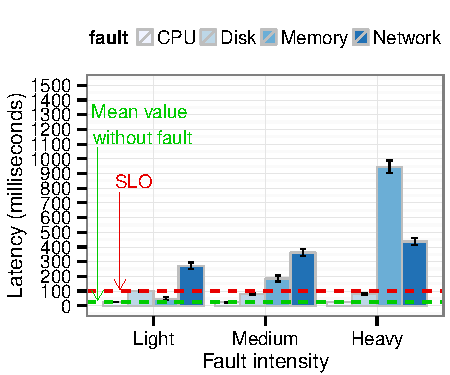
\includegraphics[width=1\textwidth]{inputs/img/fault_impact_this_latency_99th_voltdb_voter}
                \caption{99$^{th}$ percentile latency w/ Voter.}
                \label{fig:fault_impact_this_latency_99th_voltdb_voter}
        \end{subfigure}
        ~ %add desired spacing between images, e. g. ~, \quad, \qquad etc.
        \begin{subfigure}[b]{0.48\textwidth}
                  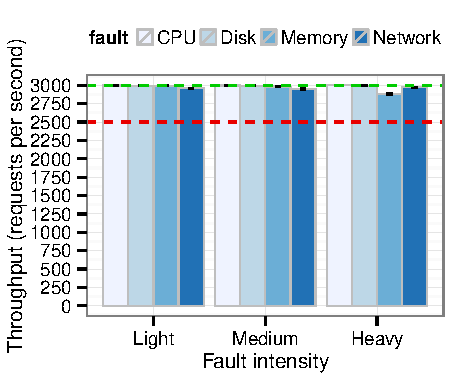
\includegraphics[width=1\textwidth]{inputs/img/fault_impact_this_throughput_voltdb_voter}
                \caption{Average throughput w/ Voter.}
                \label{fig:tejo_overview_detecting}
        \end{subfigure}

        \begin{subfigure}[b]{0.48\textwidth}
                  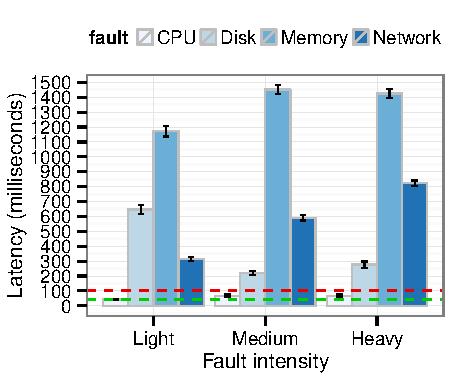
\includegraphics[width=1\textwidth]{inputs/img/fault_impact_this_latency_99th_voltdb_tpcc}
                \caption{99$^{th}$ percentile latency w/ TPC-C.}
                \label{fig:fault_impact_this_latency_99th_voltdb_tpcc}
        \end{subfigure}
	  ~
        \begin{subfigure}[b]{0.48\textwidth}
                  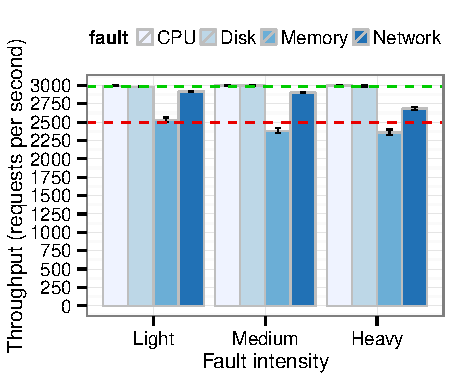
\includegraphics[width=1\textwidth]{inputs/img/fault_impact_this_throughput_voltdb_tpcc}
                \caption{Average throughput w/ TPC-C.}
                \label{fig:fault_impact_this_throughput_voltdb_tpcc}
        \end{subfigure}
        \caption{Performance anomalies in VoltDB as serving Voter and TPC-C, with a replication degree k=2.}
                \label{fig:performance_overview}


\end{figure*}


\begin{figure*}
        \centering
        \begin{subfigure}[b]{0.48\textwidth}
               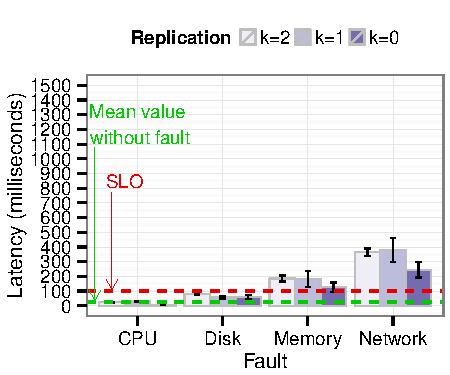
\includegraphics[width=1\textwidth]{inputs/img/k_factor_latency_99th_voltdb_k_analysis_voter}
                \caption{Voter workload.}
                \label{fig:k_factor_latency_99th_voltdb_k_analysis_voter}
        \end{subfigure}
        ~ %add desired spacing between images, e. g. ~, \quad, \qquad etc.
        \begin{subfigure}[b]{0.48\textwidth}
                  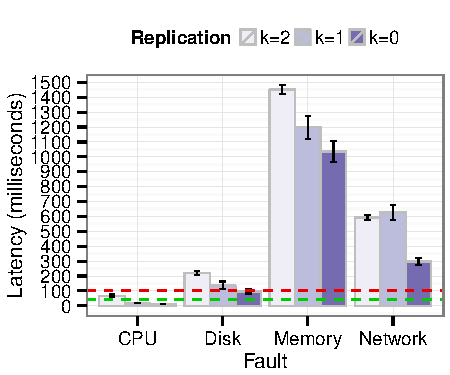
\includegraphics[width=1\textwidth]{inputs/img/k_factor_latency_99th_voltdb_k_analysis_tpcc}
                \caption{TPC-C workload.}
                \label{fig:k_factor_latency_99th_voltdb_k_analysis_tpcc}
        \end{subfigure}
        \caption{Medium fault impact on VoltDB with different k values.}
         \label{fig:replication_degree_resiliency}

\end{figure*}

\subsection{Predictive efficiency analysis}

We evaluated the predictive efficiency of learning model of Tejo with three learning algorithms, random forests, gradient boosting, and SVM. To this end, we used data derived from the dataset of Subsection~\ref{subsec:performance}. The derived data was computed by the Tejo's data handler, as described in Subsection~\ref{subsec:tejo_phases}. Each new sample had 147 features ($d=147$, as discussed in Subsection~\ref{subsec:anomaly}) and a label corresponding to a class of Tejo's learning model (see Subsection~\ref{subsec:tejo_components}). Recall that anomaly-related labels are only assigned to samples that violated the SLO. The resulting dataset contained 10,000 samples for each evaluated workload, including 5,000 of samples representing anomalous events in VMs. To validate the learning model properly, this dataset was split in two uneven parts: three-fifths of data for training the model and two-fifths for testing its predictive efficiency. We used two well-known measures to evaluate the learning model efficiency, precision and F1-score. We also computed the overhead of predictions with each learning algorithm.

Table~\ref{tab:predictive_efficiency} summarizes our results. Regardless the learning algorithm, the learning model of Tejo was able to detect 96\% of anomalies properly. It performed better with random forests algorithm, whose overall score was 0.99 (up to 1) for both precision and F1-score measures. Random forests also provided the lowest overhead for anomaly detection, requiring less than 30 microseconds for a prediction. The SVM algorithm had the worst predictive performance, particularly to detect memory-related anomalies. SVM also incurred the highest overhead for anomaly detection with our model, performing two orders of magnitude slower. According to Friedman~\cite{friedman2006recent}, this happens because SVM shares the disadvantages of ordinary kernel methods, such as poor computational scalability and inability to deal with irrelevant features. In contrast, boosting methods, like random forests and gradient boosting, overcome these issues by using a linear combination of (many) trees.

			\begin{table*}[htdp]
				\begin{center}
\caption{Anomaly detection performance with different learning algorithms.}
  \label{tab:predictive_efficiency}
					\begin{tabular}{r||c | c  c  c  | c  c  c   }
						\multirow{3}{*}{\bf Algorithm}&\multirow{3}{*}{\bf Class}& \multicolumn{6}{ c }{\bf workload} \\ \cline{3-8}
						&&\multicolumn{3}{ c | }{\bf voter}&\multicolumn{3}{ c }{\bf TPC-C} \\ \cline{3-8}
						&&precision&F1-score&overhead&precision&F1-score&overhead \\ 
						\hline
						\hline
						\multirow{3}{*}{\makecell{Random \\  Forests}}&Normal&0.99&0.99&\multirow{3}{*}{23$\mu$s}&0.98&0.99&\multirow{3}{*}{26$\mu$s} \\
						&Network&0.98&0.98&&0.99&0.98& \\
						&Memory&0.99&0.98&&0.98&0.99& \\
						&Disk&0.99&0.98&&1.00&1.00& \\
						\hline
						\multirow{3}{*}{\makecell{Gradient \\ Boosting}}&Normal&0.99&0.99&\multirow{3}{*}{30$\mu$s}&0.96&0.98&\multirow{3}{*}{33$\mu$s} \\
						&Network&0.99&0.99&&0.99&0.96& \\
						&Memory&0.99&0.99&&0.98&0.99& \\
						&Disk&1.00&1.00&&1.00&1.00& \\
						\hline
						\multirow{3}{*}{SVM}&Normal&0.98&0.97&\multirow{3}{*}{4294$\mu$s}&0.98&0.98&\multirow{3}{*}{5441$\mu$s} \\
						&Network&0.97&0.96&&0.99&0.97& \\
						&Memory&0.85&0.91&&0.87&0.93& \\
						&Disk&1.00&0.97&&1.00&1.00& \\
					\end{tabular}
				\end{center}
			\end{table*}

In addition to the predictive efficiency evaluation, Tejo allows us to analyse the importance of features using boosting methods. Figure~\ref{fig:feature_importance_plots} plots the importance of features of the Tejo's learning model, where the sum of all features importances is equal to one.  Figure~\ref{fig:feature_importance} shows the 10 most-important features for anomaly detection in VoltDB serving Voter, seven out of 10 corresponding to performance counters of TCP layer of VMs. This suggests that the peer-to-peer communication pattern among the VoltDB cluster is key for anomaly detection. To provide insights into all 147 features, we organized them into seven distinct categories and measured their grouped importance, as depicted in Figure~\ref{fig:feature_importance_categories}. Indeed, it confirms that features from TCP performance counters form the main category, accounting for more than half the total of importance (0.5345). Surprisingly, the category of VoltDB features had the lowest importance for the anomaly detection task. This suggests that the contribution of database-specific features is negligible, therefore our learning model is likely to have similar predictive performance with different NewSQL databases. Results for TPC-C workload showed a similar trend.

\begin{figure*}
        \centering
        \begin{subfigure}[b]{0.48\textwidth}
               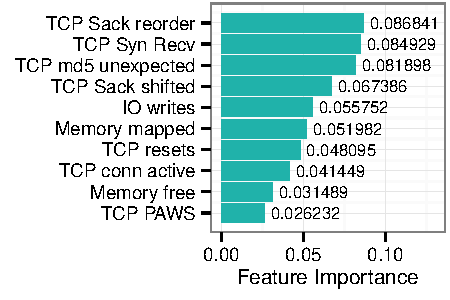
\includegraphics[width=1\textwidth]{inputs/img/feature_importance}
                \caption{The 10 most-important features.}
                \label{fig:feature_importance}
        \end{subfigure}
        ~ %add desired spacing between images, e. g. ~, \quad, \qquad etc.
        \begin{subfigure}[b]{0.48\textwidth}
                  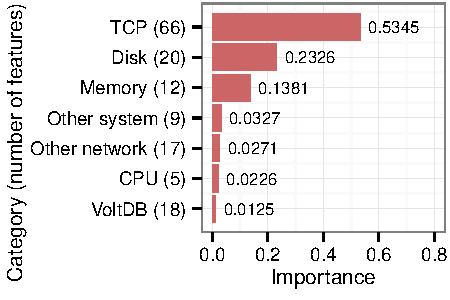
\includegraphics[width=1\textwidth]{inputs/img/feature_importance_categories}
                \caption{Importance of features categories.}
                \label{fig:feature_importance_categories}
        \end{subfigure}
        \caption{Analysis of the importance of features for anomaly detection.}
        \label{fig:feature_importance_plots}
\end{figure*}
